\documentclass[a4paper,11pt]{article}
\usepackage[utf8]{inputenc}
\usepackage[T1]{fontenc}
\usepackage[english]{babel}
\usepackage{array}
\usepackage{multirow}
\usepackage{multicol}
\usepackage{fullpage}
\usepackage{listingsutf8}
\usepackage{caption}
\usepackage{float}
\usepackage{subcaption}
\usepackage{amsmath}
\usepackage{enumitem}
\usepackage{amsthm}
\usepackage{amsfonts}
\usepackage{amssymb}
\usepackage{color}
\usepackage[nounderscore]{syntax}
\usepackage{graphicx}
\definecolor{mygreen}{rgb}{0,0.6,0}
\definecolor{mygray}{rgb}{0.5,0.5,0.5}
\definecolor{mymauve}{rgb}{0.58,0,0.82}
\usepackage{hyperref}
\usepackage[usenames,dvipsnames]{xcolor}
\hypersetup{
     colorlinks   = true,
     citecolor    = gray,
     linkcolor    = blue,
}


\newcommand\bb{Benjamin Boisson}
\newcommand\gc{Guillaume Combette}
\newcommand\dl{Dimitri Lajou}
\newcommand\vl{Victor Lutfalla}
\newcommand\om{Octave Mariotti}
\newcommand\mr{Raphaël Monat} % Okay, \rm was already taken too.
\newcommand\me{Etienne Moutot} % He is not the only one author o/ Just that \em is already taken
\newcommand\js{Johanna Seif}
\newcommand\ps{Pijus Simonaitis}



\title{Mid-year report, Blend'it project}
\author{\bb, \gc, \dl,\\ \vl, \om, \mr,\\ \me, \js, \ps}


\begin{document}

\maketitle

\begin{abstract}
This is our mid-year  report of the integrated project called ``Blend'it''. The goal of this project is to design two open-source plugins for Blender, which is a computer graphics software. One of these plugin will be able to render and animate crowds, and the other one to design environments by making different elements such as rivers and mountains automatically interact to produce realistic scenes. Although this kind of software is already developed in the Computer Graphics industry, it is often unavailable to the public and not of free use.
\end{abstract}


\tableofcontents

\newpage

\section{General overview of the project}

\subsection{Objectives}
The goal of this project is to improve the open-source 3D software Blender, by providing two new plugins. Blender can create 3D scenes from scratch, from modelling to animation and render.

The aim is to add to Blender the possibility to generate large populated environments. There are two independents parts: first generate environments in a semi-automated way. Secondly, generate and animate people of the environment, whose movements must be consistent with the environment and other people's movements.

There have been a lot of researches around the procedural generation of crowds and environments in computer graphics. But the large majority are implemented as research prototypes or in commercial software. To the best of our knowledge, nothing exists for widely used free software like Blender.

\paragraph{Related work.} The animation of large crowds is really developed in the computer graphics industry, enabling commercial 3D software to easily render massive scenes with large crowds. For example, the ILM studio developed a software called Massive (\cite{Massive}) dramatically changed the habits of 3D studios: for example, it helped generating the armies being displayed in \textit{Lord of the Rings}. The Golaem (\cite{Golaem}) software is also able to render massive crowds in different situations, and is used by the studio producing \textit{Game of Thrones}. Nowadays, even commercial standalone 3D software like 3DS MAX\cite{3dsmax} is able to generate realistic crowds. On the contrary, no open-source software provides this kind of feature. In the past, scripts had been developed, but they were not providing realistic results, and are not working anymore.

\paragraph{Choice of Blender.}

The big advantage of producing a code based on Blender is that we can use its Python API, which is very powerful. With it, one can manipulate every objects and part of the Blender interface without re-compiling blender or even modifying the source code. Thus, we can concentrate only one the new parts of the project: our algorithms, we do not need to code another render engine for example.
The other advantage is the Blender community, which already exists, and on which we can rely to have feedback on our project.



\subsection{Team and background}

We are 9 Master students from the \textit{École Normale Supérieure de Lyon}, France. As a part of our First year of Master in Research in Computer Science, we need to develop and code a project of our choice (here, ``Blend'it''), during the whole year. We are supervised by an Associate Professor from the ENS Lyon, Eddy Caron. There is a project leader, \me, and a deputy leader, \mr. Please do not hesitate to contact us, by writing an email at \textit{first name . last name @ens-lyon.fr}.\\

All our work is hosted on Github, and can be consulted on \url{github.com/blendit}.

\subsection{Work Packages}
We decided to create sub-working groups, with each group having a separate leader. We detail below the groups, the leader being in bold font.

\begin{enumerate}[label=WP\arabic*:, start=0]
\item Communication: \textbf{\mr}, \me, \js
\item Blender Code: \mr, \textbf{\me}, \ps
\item Bibliography on crowd animation: \dl, \vl, \textbf{\js}
\item Bibliography on environment generation: \bb, \textbf{\gc}, \om
\item Crowd plugin development: \dl, \vl, \me, \textbf{\js}, \ps
\item Environment plugin development: \bb, \textbf{\gc}, \om, \mr, \me,
\item Graphical User Interface (GUI) development: \gc, \textbf{\vl}, \me
\item Trailer: \dl, \textbf{\me}, \js
\end{enumerate}

\subsection{Planning}

%% TODO : ajouter le passé du planning?
Our planning for the following weeks is the following:

\begin{description}
  \item[17 Dec. - 21 Jan.] \textit{Implementation}. We plan to code the core which is the code independent from Blender, and start the design and implementation of the graphical interface.
  \item[21 Jan. - 4 Feb.] \textit{Blender part}. We will code the interface between our classes and Blender objects.
  \item[4 Feb. - 18 Feb.] \textit{Graphical interface}. We plan to refine the graphical interface to make it usable by artists. Then, depending on the defence date, we will adapt the following part of the planning.
  \item[18 Feb. - ..] \begin{itemize} \item \textit{Trailer, communication}. We will start to create examples generated by our tools, as well as communicate to and have feedback from the Blender community. \item \textit{New features}.
This will be the time to add new features note developed before like:
  \begin{itemize}
    \item People moving on non-plane surfaces
    \item Improve people animation
    \item Add more environments types
  \end{itemize}
  \end{itemize}
\end{description}


\section{WP0 - Communication}

The goal of this work package is to handle communications, both within the whole project group and with people not involved in this project (for example, the Blender community). Up to now, we have not done much: the purpose of this group is mainly to spread the software until a stable version is released. We created a forum thread on the website blenderartist (\cite{blenderartist}), to see if the blender community had special needs. We also took notes of every meeting we had on a wiki (\cite{comptesrendus}), and created a (yet really simple) website (\cite{site}). We are also responsible for the redaction and finalization of the reports (although we asked for this mid-year report every Work Package to give us a summary of their state).

\par What needs to be done next? As stated before, we plan to spread the news of the existence of this software when a stable release is published. We will probably update the website with more informations soon, and we will have to finalize the final report too.

\section{WP1 - Blender Core}

The primary goal of this work package was to explore how Python is interfaced with Blender, while Work Packages 2 and 3 were searching for articles to base our future work on. Blender is really well-interfaced with Python. Although there are not many tutorials or books talking about advanced scripting in Blender, the Blender interface can provide a Python translation of any action done in Blender with the mouse and the keyboard. This permits us to just try something by hand and then being able to implement it. 
\par Not everybody was familiar with Python at the beginning of the year, so we also devoted the major part of a meeting to an introduction to Python, and the interfacing with Blender. To ensure some consistency between us, and a certain readability of the code, we presented the PEP-8 coding convention (\cite{pep8}) to the whole group. To enforce them, we linked our Github repositories to Travis, enabling unitary tests, and rejections of code not conforming to the PEP-8.
\par We also set some strict rules on the management of Github repositories, especially concerning branches, pull-requests, etc.
\paragraph{Remaining Work.} The work of this Working Package is mostly finished: now everyone should be able to code in Python and use Blender. We will however continue to add unitary tests in order to avoid bugs and prevent regressions during development. 

\section{WP2 - Biliography on Crowd animation}

The goal of this workpackage is to find how to simulate large crowds in a rather realistic manner. After a few researches we have noticed that the crowds can be divided into two types: moving crowds and motionless crowd. We have decided focus on moving crowds. 

There are two major difficulities in moving crowds. Firstly we have to generate the path that each person will follow, and then we have to coordination the motions of the moving characters (its foot, arms, ...) with speed of the walk and the calculated path.

\paragraph{Generation of the path}

The strategy used for the crowd simulation is the least-effort approach given in \cite{PLE}.\\
In this algorithm each individual has an objectiove. The trajectory is optimized by computing the minimum energy cost in between the starting point and the arrival point (the objective). To find this minimum we use Euler's method: each timestep we compute the minimum cost path on a small distance. The ``far'' trajectory is needed for this computation, and so we approximate it using a graph containing the allowed positions on the environment, the ``far''trajectory is just a min-cost path on the graph. By iterating, this method provides us a set of points that describe the path followed by each character.

This algorithm takes into account of the velocity of each character. And the velocities are chosen so that there is no collision between two characters, and between a charactere and the environment.

The reachable points on the environnement are described by a level map, and by a set of exclusion polygones. A graph is used, as we said before, to approximate the remaining distances. Its edges are weighted by the distances between two points. Each character can go to different vertices.

In order to have an easy way to move large crowd (and not have to set individual objectives to hundreds of people) we decided to allocate to each set of character a set of interest points with a given probability to go to one of them. For the sake of simplicity, we will start with only one goal per charactere.

Moreover we thought about how to take into acount the altitude of the world. For example, if there is a mountain, it is sometime more efficiant to bypass it. The idea we had for that is to modify the weight of the edges in function of the height of the point. 

\paragraph{Motions of the characters}

The first studies were based on the article .%TODO bibliography




\section{WP3 - Environment}

The main architecture comes from \cite{DeclarativeArchitecture}. It is a
layered architecture, from large-scale features to low-scale ones. Each feature
covers a user-delimited areas, which may be further reduced because of
conflicts with the surrounding features. The modularity of the architecture
allows features to be edited independently of each other. The output may
include: an height map, a texture map and additional objects to be added on top
of this such as a water map, vegetation or buildings.
% Interface with the crowd team: summarize as an accessibility map.

The height map is generated using the tree structure described in
\cite{FeatureTree}. The conversion from the layered architecture amounts to
choosing the appropriate merging nodes: the leaves are exactly the features of
the layers. Furthermore, this representation can compute the height at any
point, allowing a greater level of detail when and where needed.

Generating cities is done in three consecutive steps: \begin{enumerate}
  \item Create the road network. This will be done using the method proposed in
    \cite{StreetTensors}, which seems to support easy edition.
  \item Divide each block into parcels, following the method given in
    \cite{PGParcels}.
  \item Generate a building in each parcel. This can be done either using
    predefined buildings or procedurally generated using L-systems, as in
    \cite{FLSystem}.
\end{enumerate}

\section{WP4 - Crowd plugin development}

\paragraph{Generation of the path}~

\noindent The algorithm of least-effort approach is divided in many points.
\begin{itemize}
  \item Grid arrangement and setting up of the grid.
  \item Computation of the minimum on a graph with the $A*$ algorithm.
  \item Computation of the authorised velocity field.
  \item Finding the exclusion zones in order to do the minimisation.
  \item Update of the graph with the attribution of a new weight on the edges: each character affect the weight of its neighbour edges.
\end{itemize}

\todoall{C’est dommage de s’arrêter en si bon chemin. Pour chaque
  itemize une description d’un paraphe pour décrire les efforts et
  avancés menés ne serait pas un luxe. Par exemple pour chaque point on peut se poser la question du comment ? }

\noindent We also started coding the classes that we will use (summarised on Figure \ref{crowd_classes}):
\begin{description}
  \item[Graph] This class describes the graph that was set up, with a set of nodes and a dictionary of dictionaries of edges.
  \item[Individual] This class describe an individual within the crowd. It includes the position, maximal speed, optimal speed, trajectory and some variables to compute the energy of the individual.
  \item[Crowd] contains a set of individuals and the graph.
  \item[Environment] gives the set of forbidden regions.
  \item[Blend*] These are the classes using Blender. They take the corresponding ``non-blend'' class and convert it into a Blender object, usable in Blender. 
\end{description}

We also try to keep as much code as possible independent from Blender. It will lead to easier tests and a more portable code from Blender to another 3D software.

\begin{figure}[h]
  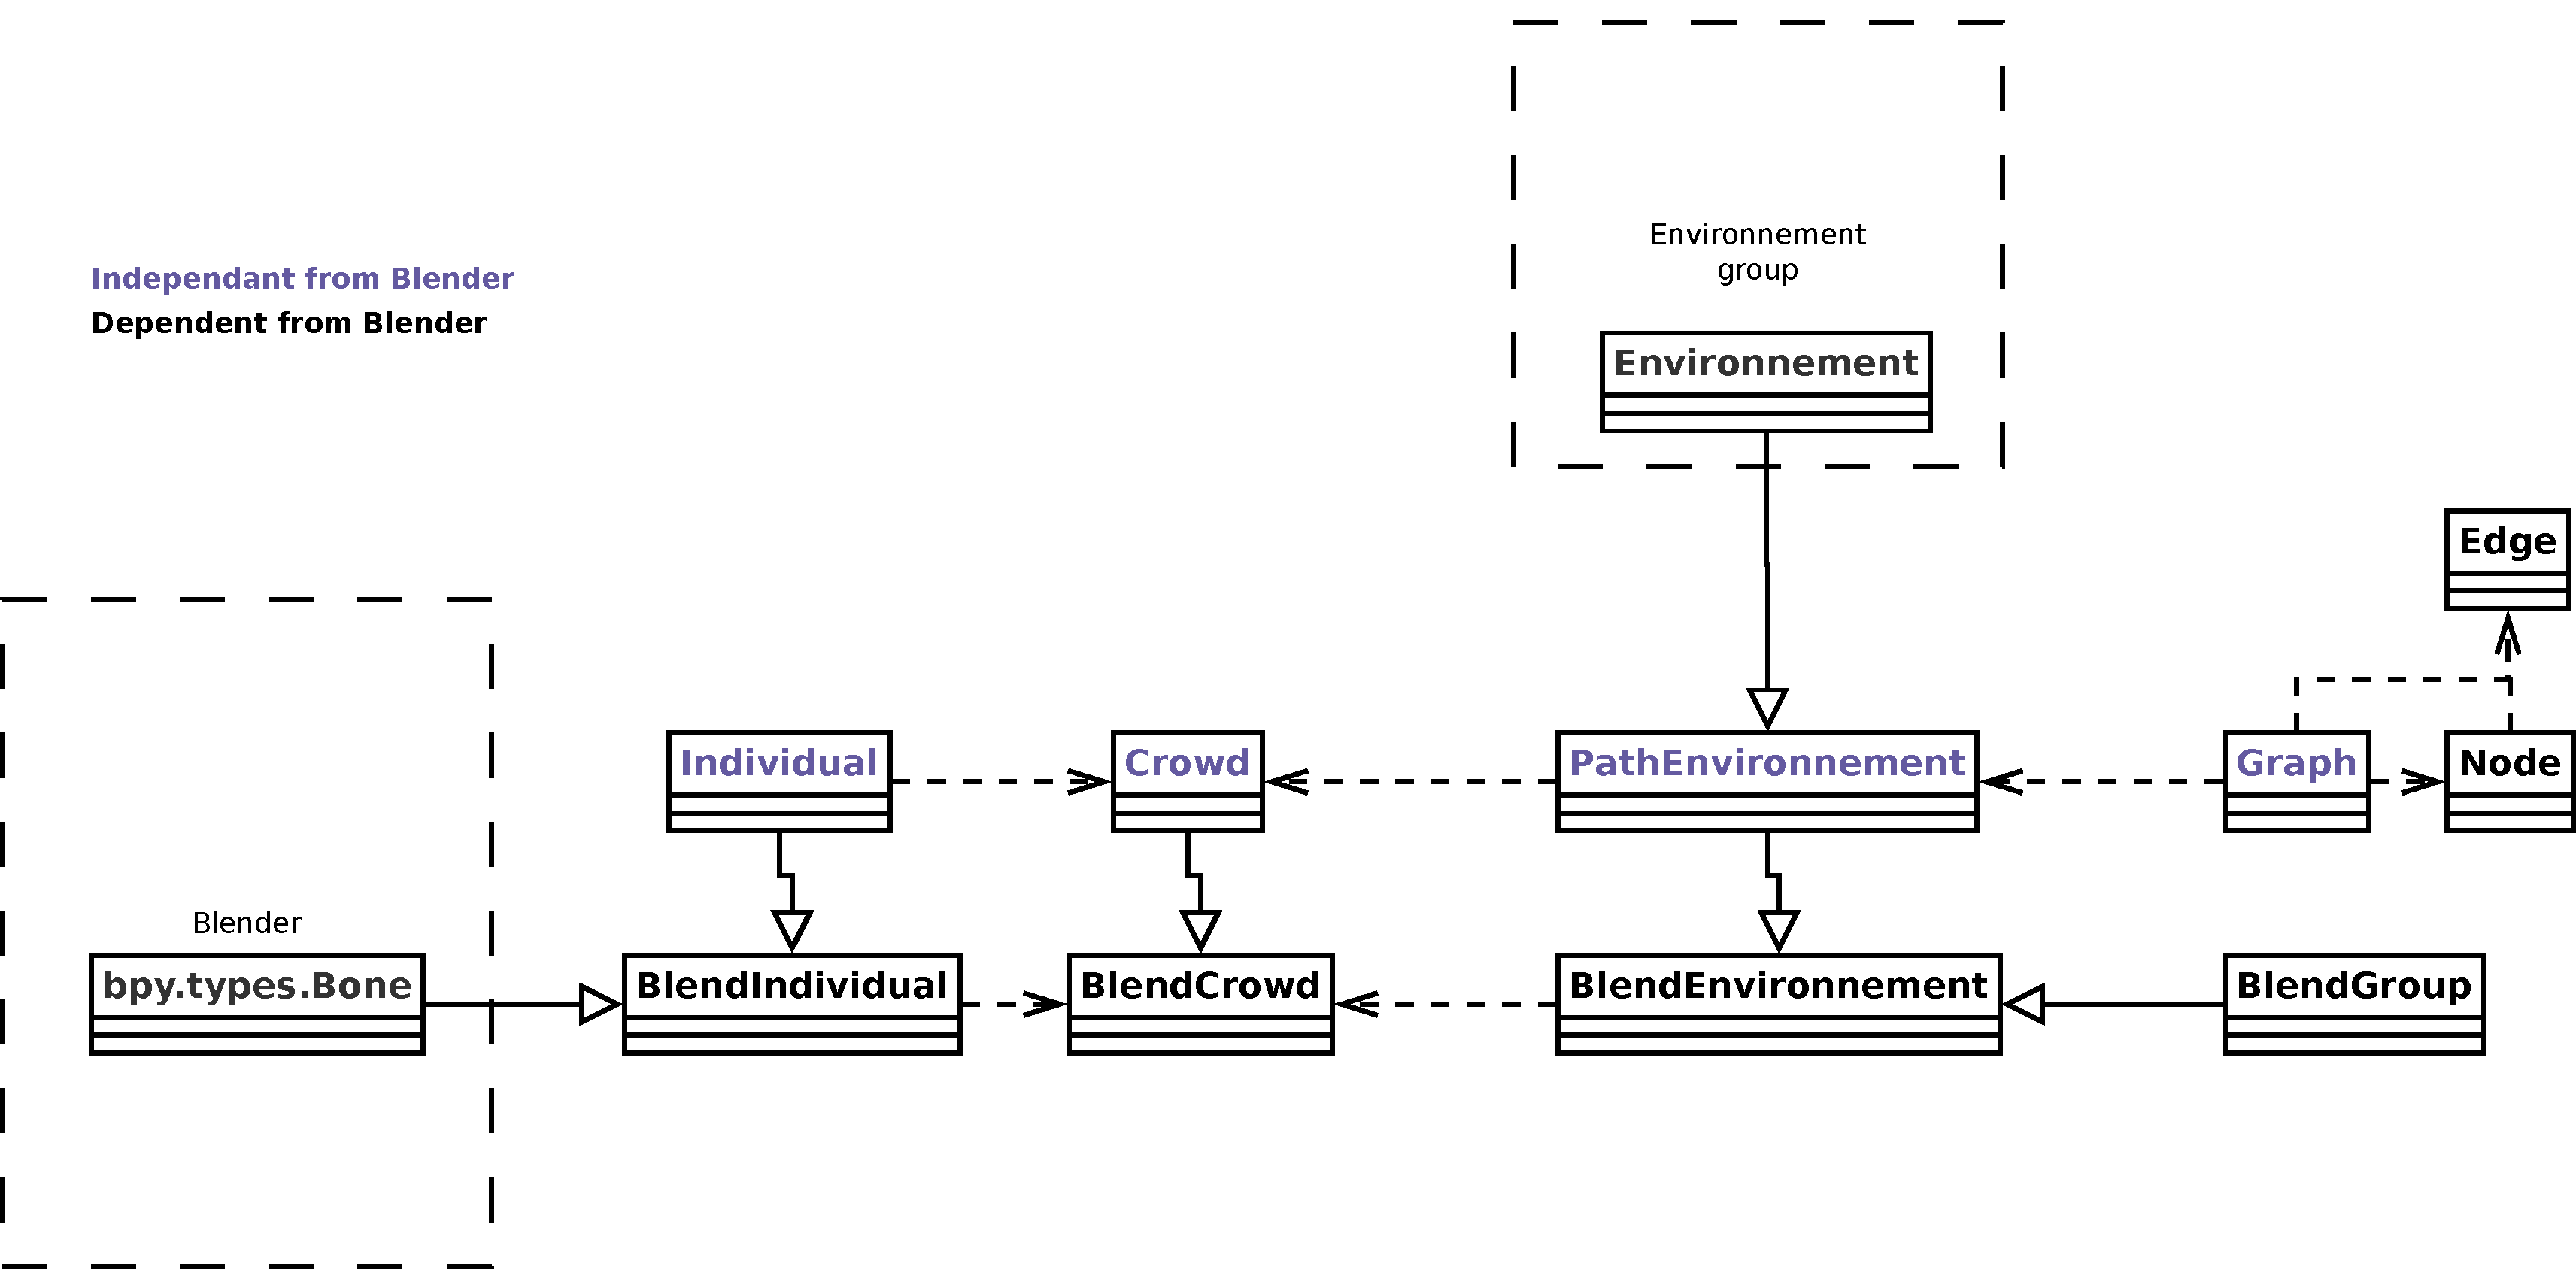
\includegraphics[width=15cm]{crowd_final.pdf}
  \caption{Classes of \texttt{crowd plug-in} and relations between them.}
  \label{crowd_classes}
\end{figure}

\paragraph{Motions of the characters}~

As stated in the paragraph \ref{WP2_motion}, the bibliographical work on the animation of characters was longer than expected and is currently being finalised: the implementation part has yet not begun.




\section{Environment plugin development (WP5)}

The articles mentioned in part \ref{WP3} describe quite precisely the algorithms usable to build and merge the different features. The work done for the code of the environment part was to organise the different algorithms into several classes (summarised on Figure \ref{env_classes}). The main classes are:

\begin{description}
  \item[Feature] This class is like an abstract class. It is the base from which every feature inherit, to allow us to manipulate generic feature in our code.
    \item[FeatureTree] This class build the tree of the features, depending on their positions and thus their interactions. It also solves the ``merge'' of the different features.
    \item[Environment] This one is the final 3D environment, which uses the 3D models and the feature tree to build the 3D environment.
    \item[BlendEnvironment] This class is the only one depending on Blender, it converts the Environment class to allow it to be displayed and used into Blender.
\end{description}

\begin{figure}[h]
  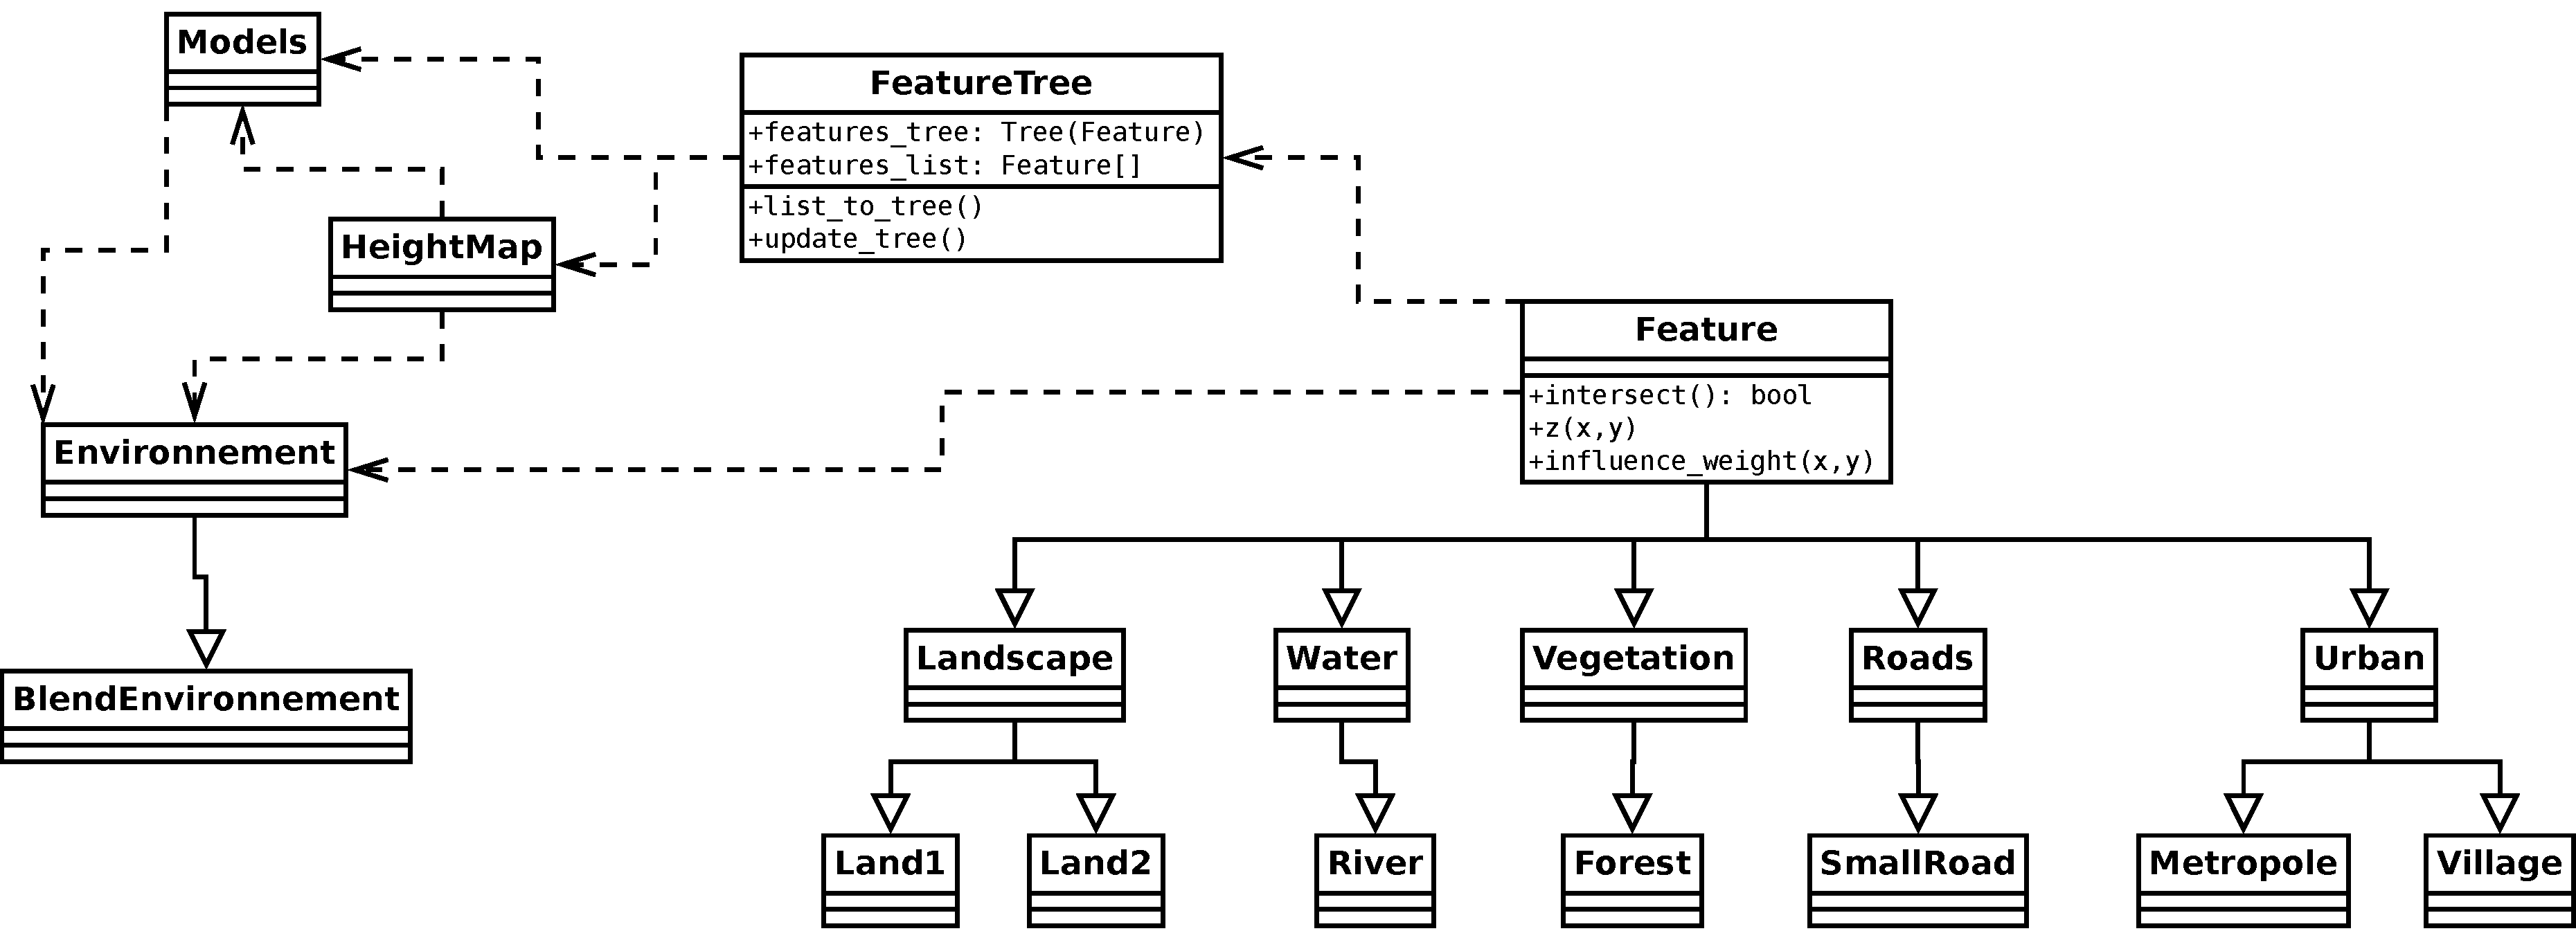
\includegraphics[width=15cm]{env_final.pdf}
  \caption{Classes of \texttt{environment plug-in} and relations between them.}
  \label{env_classes}
\end{figure}

\section{WP6 - GUI development}

The purpose of this work package is to ensure that when Graphical User Interface will be developped, they will be consistent with Blender User Interface. To do this, we will have to explore the Blender documentation, to see if some written guidelines exist. Otherwise, we will need to get in touch with the Blender community to see if our drafts of GUI will be natural to use.

\section{Trailer development}




\newpage
\begingroup

\bibliographystyle{alpha}
\bibliography{miparcours}

\endgroup

\end{document}

